\addcontentsline{toc}{section}{Appendix}
\section*{Appendix}

{\renewcommand{\arraystretch}{1.5}
\begin{table}[H]
\begin{center}
\begin{tabular}{rccccc}
\hline
\hline
\multirow{2}{*}{Country} & \multirow{2}{*}{Equity} & \multirow{2}{*}{Bills} & GDP & Consumption & \multirow{2}{*}{Inflation}\\
& & & (per capita) & (per capita) &\\
\hline

Australia & 1870-2015 & 1870-2015 & 1870-2015 & 1870-2015 & 1870-2015 \\ 

Belgium & 1870-2015 & 1870-2015 & 1870-2015 & 1913-2015 & 1870-2015 \\ 

Denmark & 1873-2015 & 1875-2015 & 1870-2015 & 1870-2015 & 1870-2015 \\ 

Finland & 1896-2015 & 1870-2015 & 1870-2015 & 1870-2015 & 1870-2015 \\ 

France & 1870-2015 & 1870-2015 & 1870-2015 & 1870-2015 & 1870-2015 \\ 

Germany & 1870-2015 & 1870-2015 & 1870-2015 & 1870-2015 & 1870-2015 \\ 

Italy & 1870-2015 & 1885-2015 & 1870-2015 & 1870-2015 & 1870-2015 \\ 

Japan & 1886-2015 & 1876-2015 & 1870-2015 & 1870-2015 & 1870-2015 \\ 

Netherlands & 1900-2015 & 1870-2015 & 1870-2015 & 1870-2015 & 1870-2015 \\ 

Norway & 1881-2015 & 1870-2015 & 1870-2015 & 1870-2015 & 1870-2015 \\ 

Portugal & 1871-2015 & 1880-2015 & 1870-2015 & 1910-2015 & 1870-2015 \\ 

Spain & 1900-2015 & 1870-2015 & 1870-2015 & 1870-2015 & 1870-2015 \\ 

Sweden & 1871-2015 & 1870-2015 & 1870-2015 & 1870-2015 & 1870-2015 \\ 

Switzerland & 1900-2015 & 1900-2015 & 1870-2015 & 1870-2015 & 1870-2015 \\ 

United Kingdom & 1871-2015 & 1870-2015 & 1870-2015 & 1870-2015 & 1870-2015 \\ 

United States & 1872-2015 & 1870-2015 & 1870-2015 & 1870-2015 & 1870-2015 \\ 
\hline 
\hline
\end{tabular} 
\end{center}
\caption{Data coverage}
\label{tab:data_coverage}
\end{table}

{\renewcommand{\arraystretch}{1.0}
\begin{table}[H]
\begin{center}
\begin{tabular}{rccccccccccc}
\hline
\hline
Country & \multicolumn{5}{c}{Full sample (1870-2015)} & & \multicolumn{5}{c}{post-1984} \\
%\cline{2-6} \cline{8-12}
\hline
 & \multicolumn{2}{c}{Equity} & & \multicolumn{2}{c}{Bills} & & \multicolumn{2}{c}{Equity} & & \multicolumn{2}{c}{Bills}\\
\cline{2-3} \cline{5-6} \cline{8-9} \cline{11-12}
 & Mean & Std & & Mean & Std & & Mean & Std & & Mean & Std\\
\hline
Australia & 8.57 & 16.49 & & 1.98 & 4.47 & & 8.75 & 18.94 & & 3.62 & 2.48\\
Belgium & 5.99 & 22.92 & & 0.08 & 12.61 & & 11.92 & 24.90 & & 2.24 & 2.87 \\
Denmark & 7.89 & 17.41 & & 2.99 & 5.61 & & 10.84 & 21.53 & & 2.70 & 3.17 \\
Finland & 8.90 & 33.26 & & -1.45 & 14.90 & & 15.74 & 42.53 & & 2.84 & 3.65\\
France & 3.02 & 23.67 & & -1.32 & 9.58 & & 10.47 & 24.49 & & 2.45 & 2.71\\
Germany & 7.89 & 30.56 & & -2.57 & 27.64 & & 10.31 & 24.72 & & 1.86 & 1.92\\
Italy & 5.55 & 29.71& & -0.95 & 16.26 & & 9.99 & 29.99 & & 2.86 & 2.94\\
Japan & 6.83 & 35.76 & & -2.41 & 23.90 & & 5.46 & 22.63 & & 1.26 & 1.90\\
Netherlands & 7.26 & 22.65 & & 0.75 & 4.92 & & 10.69 & 22.81 & & 2.03 & 2.56 \\
Norway & 5.81 & 20.72 & & 0.81 & 6.04 & & 12.55 & 28.90 & & 2.19 & 1.86\\
Portugal & 3.87 & 28.93 & & -0.28 & 10.50 & & 11.41 & 39.75 & & 1.97 & 2.94 \\
Spain & 6.00 & 22.28 & & -0.37 &  7.15 & & 14.23 & 28.66 & & 2.39 & 3.54\\
Sweden & 8.17 & 20.45 & & 1.72 & 5.65 & & 13.55 & 28.24 & & 1.80 & 1.73\\
Switzerland & 6.50 & 19.41 & & 0.73 & 5.00 & & 10.12 & 22.53 & & 0.73 & 1.72 \\
United Kingdom & 7.11 & 19.37 & & 1.17 & 4.89 & & 8.67 & 15.64 & & 2.92 & 3.14\\
United States & 8.43 & 19.00 & & 2.15 & 4.62 & & 9.59 & 16.85 & & 1.67 & 2.36 \\
\hline
Average & 6.74 & - & & 0.20 & - & & 10.89 & - & & 2.22 & -\\
\hline
\hline
\end{tabular} 
\end{center}
\caption{Real rates of return (country-level), \%}
\label{tab:real_returns_countries}
\end{table}

{\renewcommand{\arraystretch}{1.0}
\begin{table}[H]
\begin{center}
\begin{tabular}{rccccc}
\hline
\hline
& \multicolumn{2}{c}{Equally weighted} & & \multicolumn{2}{c}{real GDP-weighted} \\
\cline{2-3} \cline{5-6}
& GDP & consumption & & GDP & consumption\\
\hline
Full sample & & & & &\\
\hline
Mean growth rate p.a. & 1.95 & 1.73 & & 1.93 & 1.70\\
Std.dev. & 1.17 & 1.39 & & 1.06 & 1.29\\
Geometric mean & 1.95 & 1.72 & & 1.93 & 1.70\\
Median & 1.97 & 1.84 & & 1.95 & 1.87\\
Max & 4.39 & 4.10 & & 4.09 & 4.02\\
Min & 0.21 & -1.26 & & 0.30 & -0.46\\
Kurtosis & 2.47 & 2.26 & & 2.13 & 1.89\\
\hline
Post-1984 & & & & &\\
\hline
Mean growth rate p.a. & 1.49 & 1.43 & & 1.51 & 1.59\\
Std.dev. & 0.78 & 0.69 & & 0.72 & 0.70\\
Geometric mean & 1.48 & 1.42 & & 1.51 & 1.59\\
Median & 1.96 & 1.79 & & 1.82 & 1.98\\
Max & 2.24 & 2.10 & & 2.43 & 2.42\\
Min & 0.21 & 0.24 & & 0.46 & 0.52\\
Kurtosis & 1.74 & 1.91 & & 1.50 & 1.61\\
\hline
\hline
\end{tabular} 
\end{center}
\caption{Global growth rates (1900-2015), \%, HP-filtered ($\lambda=100$)}
\label{tab:global_growth_HP}
\end{table}

{\renewcommand{\arraystretch}{1.0}
\begin{table}[H]
\begin{center}
\begin{tabular}{rccccccccccc}
\hline
\hline
Country & \multicolumn{5}{c}{Full sample (1870-2015)} & & \multicolumn{5}{c}{post-1984} \\
%\cline{2-6} \cline{8-12}
\hline
 & \multicolumn{2}{c}{GDP} & & \multicolumn{2}{c}{consumption} & & \multicolumn{2}{c}{GDP} & & \multicolumn{2}{c}{Consumption}\\
\cline{2-3} \cline{5-6} \cline{8-9} \cline{11-12}
 & Mean & Std & & Mean & Std & & Mean & Std & & Mean & Std\\
\hline
Australia & 1.45 & 1.30 & & 1.16 & 1.60 & & 1.83 & 0.51 & & 1.76 & 0.61\\
Belgium$^{*}$ & 1.66 & 2.10 & & 1.68 & 2.10 & & 1.41 & 0.68 & & 1.17 & 0.71 \\
Denmark & 1.69 & 1.06 & & 1.37 & 0.78 & & 1.06 & 0.64 & & 0.78 & 0.48 \\
Finland & 2.09 & 1.39 & & 2.12 & 1.39 & & 1.50 & 1.17 & & 1.80 & 0.77\\
France & 1.64 & 2.01 & & 1.42 & 2.10 & & 1.24 & 0.65 & & 1.23 & 0.52\\
Germany & 1.67 & 2.38 & & 1.67 & 2.31 & & 1.61 & 0.32 & & 1.30 & 0.64\\
Italy & 1.84 & 1.78 & & 1.49 & 1.97 & & 1.24 & 1.65 & & 0.82 & 1.49\\
Japan$^{*}$ & 2.46 & 2.64 & & 2.18 & 3.23 & & 1.42 & 1.05 & & 1.58 & 0.91\\
Netherlands & 1.57 & 1.72 & & 1.43 & 1.80 & & 1.60 & 0.84 & & 1.02 & 1.05 \\
Norway & 2.10 & 1.15 & & 1.84 & 0.81 & & 1.73 & 1.12 & & 2.16 & 0.64\\
Portugal$^{*}$ & 1.88 & 1.79 & & 2.36 & 1.94 & & 1.63 & 1.53 & & 2.17 & 1.91 \\
Spain & 1.81 & 1.98 & & 1.51 &  2.18 & & 1.84 & 1.58 & & 1.32 & 1.57\\
Sweden & 2.02 & 0.91 & & 1.80 & 0.72 & & 1.51 & 0.58 & & 1.14 & 0.42\\
Switzerland & 1.38 & 1.07 & & 1.27 & 0.90 & & 0.94 & 0.27 & & 0.80 & 0.17\\
United Kingdom & 1.39 & 0.81 & & 1.32 & 0.97 & & 1.66 & 0.82 & & 1.95 & 1.12\\
United States & 1.94 & 1.33 & & 1.77 & 1.04 & & 1.53 & 0.65 & & 1.81 & 0.64 \\
\hline
Average & 1.79 & - & &  & - & & 1.49 & - & &  & -\\

\hline
\hline
\multicolumn{12}{c}{$^{*}$ Belgium: 1914-2015, Japan: 1875-2015, Portugal: 1911-2015}
\end{tabular} 
\end{center}
\caption{Real growth rates (country-level), \%, HP-filtered ($\lambda=100$)}
\label{tab:real_growth_countries_HP}
\end{table}

%\begin{python}
%\caption{Peak-to-trough code}
%\label{code}
%\end{python}

\begin{python}
data = pd.read_excel(<ENTER DATASET HERE>, sheet_name = 'C JST')
data['year'] = data['C pc']
del data['C pc']
data = data.iloc[1:]
data.set_index('year', inplace=True, drop=True)
start_year = 1870
end_year = 2015
data = data.loc[start_year:end_year];
threshold = 0.095
countries = list(data.columns)
years = list(data.index)
data_pct = data.pct_change()
cons_df = data_pct
country_list = []
disaster_df_list = []
for country in countries:
    country_dict = {}
    sub_frame = data_pct[country]
    total_years = len(sub_frame.dropna())
    sub_frame_less = sub_frame.iloc[1:]
    na_index = sub_frame_less.loc[pd.isna(sub_frame_less)].index
    succession_counter = 0
    succession_container = []
    succession_year_container = []
    
    for x in years:
        if x+1 <= end_year and sub_frame.loc[x] < 0 and sub_frame.loc[x+1] < 0:
        
        	succession_counter += 1
            if succession_counter == 1:
                
                empty_list = [sub_frame.loc[x], sub_frame.loc[x+1]]
                empty_year_list = [x, x+1]
                
            elif succession_counter > 1:
                
                empty_list.append(sub_frame.loc[x+1])
                empty_year_list.append(x+1)
                
            succession_container.append(empty_list)
            succession_year_container.append(empty_year_list)
                   
        else:
      
            succession_counter = 0
        
    unique_periods = list(succession_year_container for succession_year_container,_ in itertools.groupby(succession_year_container))
    
    cumulative_contractions = []
    
    for i in list(succession_container for succession_container,_ in itertools.groupby(succession_container)):
        
        cumulative_contractions.append(sum(i))
        
    empty_check_list = []

    for idx, i in enumerate(cumulative_contractions):
    
        empty_dict = {}
    
        if i <= - threshold:
        
            empty_dict['contraction'] = i
            empty_dict['index'] = idx
			empty_check_list.append(empty_dict)
            
    disaster_df = pd.DataFrame(empty_check_list)
            
    disaster_periods = []

    for i in list(disaster_df['index'].values):
    
        disaster_periods.append(unique_periods[i])
        
    disaster_df['period'] = disaster_periods
    disaster_df['country'] = country
        
    flat_list = []
    for sublist in disaster_periods:
        for item in sublist:
            flat_list.append(item)          
            
    single_years = sub_frame[sub_frame <= - threshold]
    single_year_list = []

    for idx, i in enumerate(single_years.index):
    
        if i not in flat_list:
        
            single_year_list.append(i)
    
    left_over_df = pd.DataFrame(single_years[single_year_list])
    left_over_df.reset_index(drop = False, inplace = True)
    left_over_df.columns = ['period', 'contraction']
    left_over_df['country'] = country
    del disaster_df['index']
    final_df = disaster_df.append(left_over_df)
    final_df.reset_index(inplace=True, drop = True)
    disaster_df_list.append(final_df)
    total_number_disasters = len(final_df)
    flattened_years = []

    for i in range(len(final_df)):
    
        sub_years = final_df['period'][i]
    
        if type(sub_years) != int:
        
            sub_years = [str(item) for item in sub_years]
        
            for x in sub_years:
            
                flattened_years.append(x)
        
        elif type(sub_years) == int:
        
            flattened_years.append(str(sub_years))
            
    total_number_disaster_years = len(flattened_years)
    average_disaster_size = abs(final_df['contraction'].mean())
    non_disaster_years = total_years-total_number_disaster_years
    disaster_probability = total_number_disasters / non_disaster_years
    
    country_dict['Country'] = country
    country_dict['no disasters'] = total_number_disasters
    country_dict['no disaster years'] = total_number_disaster_years
    country_dict['average disaster size'] = average_disaster_size
    country_dict['no non-disaster years'] = non_disaster_years
    country_dict['disaster probability'] = disaster_probability
    country_dict['annual average growth rate'] = sub_frame.mean()
    country_dict['standard deviation annual growth rate'] = sub_frame.std()
    country_dict['kurtosis'] = sub_frame.kurtosis()
    country_dict['total years'] = total_years
    country_dict['missing years'] = np.NaN
    country_dict['number missing years'] = np.NaN
    
    if len(na_index) != 0:
        
        missing_years = sub_frame_less.loc[na_index]
        country_dict['missing years'] = list(sub_frame_less.loc[na_index].index)
        country_dict['number missing years'] = len(missing_years)
  
    country_list.append(country_dict)
    
consumption_disaster_df = pd.DataFrame(country_list)
consumption_disaster_events = pd.concat(disaster_df_list)
\end{python}
\begin{lstlisting}[frame=none,caption={Peak-to-trough algorithm},captionpos=b,label=lst:code]
\end{lstlisting}



{\renewcommand{\arraystretch}{1.0}
\begin{table}[H]
\begin{center}
\begin{tabular}{rccccc}
\hline
\hline
\multirow{3}{*}{Country} & \multirow{3}{*}{\shortstack{No.\\disasters}} & \multirow{3}{*}{\shortstack{No.\\disaster\\years}} & \multirow{3}{*}{\shortstack{No. non-\\disaster\\years}} & \multirow{3}{*}{\shortstack{Disaster\\probability\\(\%)}} & \multirow{3}{*}{\shortstack{Average\\disaster size\\(\%)}}\\
& & & & &\\
& & & & &\\
\hline
Australia & 4 & 15 & 130 & 3.08 & 18.18\\
Belgium$^{*}$ & 5 & 13 & 132 & 3.79 & 27.59\\
Denmark & 2 & 4 & 141 & 1.42 & 18.50\\
Finland & 5 & 15 & 130 & 3.85 & 15.48\\
France & 7 & 21 & 124 & 5.65 & 19.11\\
Germany & 4 & 14 & 131 & 3.05 & 44.03\\
Italy & 2 & 8 & 137 & 1.46 & 36.17\\
Japan$^{*}$ & 2 & 8 & 137 & 1.46 & 35.19\\
Netherlands & 3 & 15 & 130 & 2.31 & 35.92\\
Norway & 3 & 6 & 139 & 2.16 & 13.23\\
Portugal$^{*}$ & 2 & 3 & 142 & 1.41 & 13.14\\
Spain & 4 & 13 & 132 & 3.03 & 16.73\\
Sweden & 3 & 5 & 140 & 2.14 & 11.90\\
Switzerland & 3 & 9 & 136 & 2.21 & 16.09\\
United Kingdom & 2 & 7 & 138 & 1.45 & 18.05\\
United States & 5 & 13 & 132 & 3.79 & 16.45\\
\hline
$\Sigma$ & 56 & 169 & 2,151 & 2.60 & $\mu=22.23$\\
\hline
\hline
\multicolumn{6}{c}{$^{*}$ Belgium: 1914-2015, Japan: 1875-2015, Portugal: 1911-2015}
\end{tabular} 
\end{center}
\caption{Disaster risk moments (GDP)}
\label{tab:disaster_risk_gdp}
\end{table}

\begin{figure}[H]
	\centering
  \includegraphics[width=\textwidth]{Graphics/Gantt_GDP_highres.PNG}
	\caption{GDP disasters across countries over time}
	\label{fig:Gant_GDP}
\end{figure}

{\renewcommand{\arraystretch}{1.0}
\begin{table}[H]
\begin{center}
\begin{tabular}{rccccc}
\hline
\hline
Country & \multicolumn{2}{c}{Consumption} & & \multicolumn{2}{c}{GDP} \\
%\cline{2-6} \cline{8-12}
\cline{2-3} \cline{5-6} 
 & $g$ & $\sigma$ & & $g$ & $\sigma$\\
\hline
Australia & 2.51 & 4.41 &  & 2.28 & 3.44\\
Belgium & 3.46 & 6.34 &  & 3.17 & 7.03\\
Denmark & 2.08 & 4.36 &  & 2.07 & 3.13\\ 
Finland & 3.36 & 4.31 &  & 3.02 & 3.69\\ 
France & 2.41 & 5.30 &  & 3.24 & 4.94\\ 
Germany & 3.08 & 4.22 &  & 3.66 & 4.20\\
Italy & 1.83 & 3.35 &  & 2.56 & 3.58\\
Japan & 3.18 & 5.41 &  & 3.28 & 4.77\\
Netherlands & 2.82 & 6.89 &  & 2.83 & 6.57\\
Norway & 2.37 & 3.11 &  & 2.56 & 3.06\\ 
Portugal & 3.20 & 3.82 &  & 2.17 & 3.98\\
Spain & 4.24 & 5.52 &  & 2.70 & 4.11\\
Sweden & 2.17 & 4.04 &  & 2.43 & 2.81\\
Switzerland & 2.36 & 5.22 &  & 1.95 & 3.45\\
United Kingdom & 1.71 & 2.32 &  & 1.78 & 2.43\\
United States & 2.23 & 3.11 &  & 2.87 & 4.12\\
\hline
\hline
\end{tabular} 
\end{center}
\caption{Growth rates (non-disaster years), \%}
\label{tab:growth_non_disaster}
\end{table}

{\renewcommand{\arraystretch}{1.0}
\begin{table}[H]
\begin{center}
\begin{tabular}{rccccccc}
\hline
\hline
Country & $g^{*}$ (\%) & $\rho^{*}$ & $\beta^{*}$ & $r^{e}$ (\%) & $r^{f}$ (\%) & \underline{$\gamma$} & \boldsymbol{$\gamma$}\\
\hline

Australia & 1.78 & 0.0414 & 0.9603 & 6.98 & 2.58 & 39.18 & 9.58\\ 

Belgium & 2.37 & 0.0328 & 0.9683 & 7.30 & 3.36 & 8.88 &  3.51\\ 

Denmark & 1.86 & -0.0142 & 1.0144 & 6.80 & 3.54 & 36.61 &  10.94\\ 

Finland & 2.50 & 0.0529 & 0.9498 & 7.76 & 0.86 & 50.99 &  13.42\\ 

France & 2.28 & 0.0115 & 0.9887 & 7.04 & 4.15 & 11.10 &  4.59\\ 

Germany & 2.40 & 0.0501 & 0.9523 & 7.61 & 0.64 & 16.70 &  3.03\\ 

Italy & 2.10 & 0.0248 & 0.9758 & 7.03 & 2.70 & 29.69 &  4.65\\ 

Japan & 2.88 & 0.0106 & 0.9895 & 7.72 & 1.56 & 25.89 &  5.44\\ 

Netherlands & 2.21 & 0.0385 & 0.9629 & 7.23 & 2.89 & 11.94 &  3.37\\ 

Norway & 2.32 & -0.0872 & 1.0956 & 7.09 & 3.75 & 39.36 &  14.57\\ 

Portugal & 2.07 & -0.0413 & 1.0431 & 6.93 & 4.16 & 22.95 &  12.12\\ 

Spain & 2.28 & -0.0003 & 1.0003 & 7.26 & 3.02 & 26.49 &  9.87\\ 

Sweden & 2.21 & -0.0628 & 1.0670 & 7.17 & 2.87 & 56.16 &  19.50\\ 

Switzerland & 1.66 & 0.0345 & 0.9667 & 6.84 & 3.00 & 38.42 &  11.77\\ 

United Kingdom & 1.55 & 0.0231 & 0.9774 & 6.69 & 2.73 & 72.30 &  12.96\\ 

United States & 2.33 & -0.0015 & 1.0015 & 7.28 & 3.10 & 26.47 &  9.19\\
\hline
Global & & & & & & &\\
\hline 
\hline
\end{tabular} 
\end{center}
\caption{Calibration \& results (GDP)}
\label{tab:results_GDP}
\end{table}

\begin{figure}[H]
	\begin{tabular}{cc}
	\subfloat[Expected rates of return on equity]{
		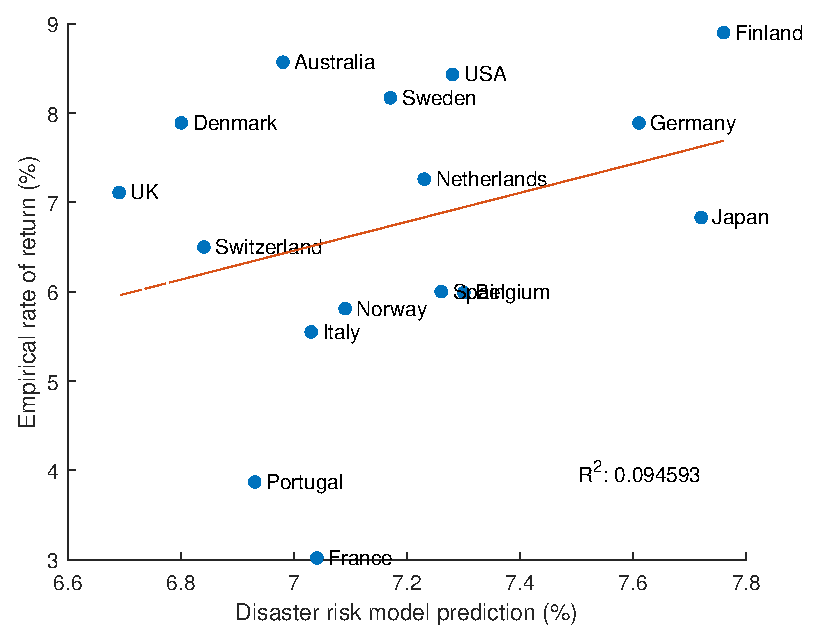
\includegraphics[width = 0.45\textwidth]{Matlab Graphics/Actual_vs_predicted_equity_GDP}
	} &
	\subfloat[Risk-free rates]{
		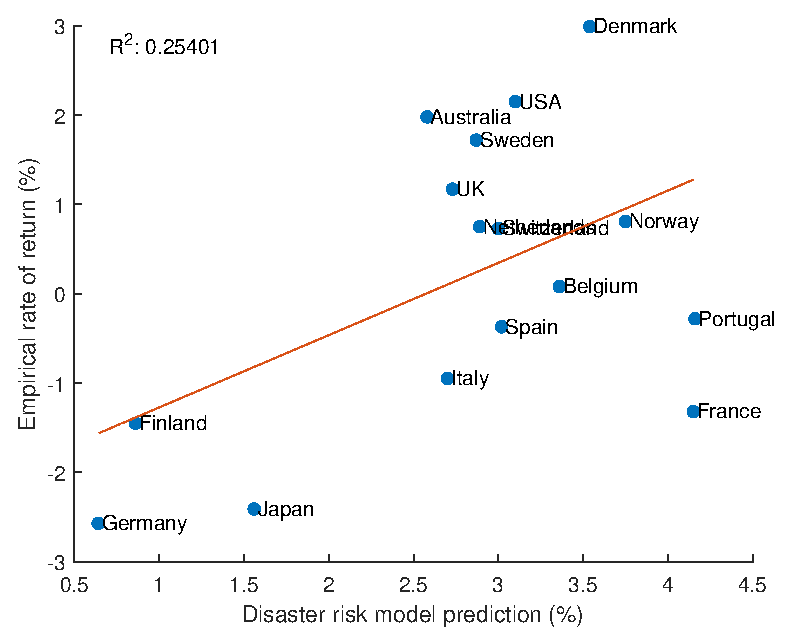
\includegraphics[width = 0.45\textwidth]{Matlab Graphics/Actual_vs_predicted_riskfree_GDP}
	}\\
	\end{tabular}
	\caption{Actual vs. predicted rates of return (GDP data)}
	\label{fig:actual_vs_predicted_rates_GDP}
\end{figure}

{\renewcommand{\arraystretch}{1.0}
\begin{table}[H]
\begin{center}
\begin{tabular}{rccccc}
\hline
\hline
\multirow{3}{*}{Country} & \multirow{3}{*}{\shortstack{No.\\disasters}} & \multirow{3}{*}{\shortstack{No.\\disaster\\years}} & \multirow{3}{*}{\shortstack{No. non-\\disaster\\years}} & \multirow{3}{*}{\shortstack{Disaster\\probability\\(\%)}} & \multirow{3}{*}{\shortstack{Average\\disaster size\\(\%)}}\\
& & & & &\\
& & & & &\\
\hline
\multicolumn{6}{c}{Consumption}\\
\hline
Australia & 6 & 17 & 128 & 4.69 & 22.60\\
Belgium$^{*}$ & 3 & 8 & 94 & 3.19 & 42.82\\
Denmark & 2 & 4 & 141 & 1.42 & 26.20\\
Finland & 3 & 10 & 135 & 2.22 & 27.85\\
France & 2 & 8 & 137 & 1.46 & 49.83\\
Germany & 2 & 12 & 133 & 1.50 & 50.82\\
Italy & 1 & 5 & 140 & 0.71 & 32.13\\
Japan$^{*}$ & 1 & 8 & 133 & 0.75 & 90.35\\
Netherlands & 3 & 10 & 135 & 2.22 & 42.14\\
Norway & 2 & 4 & 141 & 1.42 & 16.88\\
Portugal$^{*}$ & 1 & 5 & 100 & 1.00 & 23.47\\
Spain & 5 & 16 & 129 & 3.88 & 24.18\\
Sweden & 1 & 3 & 142 & 0.70 & 16.43\\
Switzerland & 4 & 11 & 134 & 2.99 & 19.52\\
United Kingdom & 2 & 8 & 137 & 1.46 & 17.72\\
United States & 2 & 8 & 137 & 1.46 & 20.02\\
\hline
$\Sigma$ & 40 & 137 & 2,096 & 1.90 & $\mu=32.69$\\
\hline
 & & & & & \\
  & & & & & \\
\hline
\multicolumn{6}{c}{GDP}\\
\hline
Australia & 3 & 10 & 135 & 2.22 & 20.45\\
Belgium$^{*}$ & 4 & 9 & 136 & 2.94 & 31.44\\
Denmark & 1 & 2 & 143 & 0.70 & 25.43\\
Finland & 1 & 2 & 143 & 0.70 & 29.94\\
France & 5 & 12 & 133 & 3.76 & 21.86\\
Germany & 3 & 13 & 132 & 2.27 & 54.14\\
Italy & 2 & 8 & 137 & 1.46 & 36.17\\
Japan$^{*}$ & 1 & 6 & 139 & 0.72 & 60.88\\
Netherlands & 2 & 10 & 135 & 1.48 & 47.09\\
Norway & 1 & 2 & 143 & 0.70 & 15.31\\
Portugal$^{*}$ & 1 & 2 & 143 & 0.70 & 15.40\\
Spain & 1 & 3 & 142 & 0.70 & 32.86\\
Sweden & 1 & 2 & 143 & 0.70 & 15.39\\
Switzerland & 2 & 6 & 139 & 1.44 & 17.55\\
United Kingdom & 2 & 7 & 138 & 1.45 & 18.05\\
United States & 2 & 7 & 138 & 1.45 & 24.80\\
\hline
$\Sigma$ & 32 & 101 & 2,219 & 1.44 & $\mu=29.17$\\
\hline
\hline
\multicolumn{6}{c}{$^{*}$ Belgium: 1914-2015, Japan: 1875-2015, Portugal: 1911-2015}
\end{tabular} 
\end{center}
\caption{Disaster risk moments (disaster threshold = 0.15)}
\label{tab:disaster_risk_threshold}
\end{table}


{\renewcommand{\arraystretch}{1.0}
\begin{table}[H]
\begin{center}
\begin{tabular}{rccccc}
\hline
\hline
\multirow{3}{*}{Country} & \multirow{3}{*}{\shortstack{No.\\disasters}} & \multirow{3}{*}{\shortstack{No.\\disaster\\years}} & \multirow{3}{*}{\shortstack{No. non-\\disaster\\years}} & \multirow{3}{*}{\shortstack{Disaster\\probability\\(\%)}} & \multirow{3}{*}{\shortstack{Average\\disaster size\\(\%)}}\\
& & & & &\\
& & & & &\\
\hline
\multicolumn{6}{c}{Consumption}\\
\hline
Australia & 2 & 26 & 119 & 1.68 & 19.01\\
Belgium$^{*}$ & 1 & 12 & 90 & 1.11 & 32.44\\
Denmark & - & - & - & - & -\\
Finland & - & - & - & - & -\\
France & 1 & 13 & 132 & 0.76 & 34.17\\
Germany & 2 & 20 & 125 & 1.60 & 21.67\\
Italy & 2 & 25 & 120 & 1.67 & 11.20\\
Japan$^{*}$ & 1 & 18 & 123 & 0.81 & 53.38\\
Netherlands & 1 & 10 & 135 & 0.74 & 20.88\\
Norway & - & - & - & - & -\\
Portugal$^{*}$ & 1 & 8 & 97 & 1.03 & 9.57\\
Spain & 1 & 12 & 133 & 0.75 & 26.90\\
Sweden & - & - & - & - & -\\
Switzerland & - & - & - & - & -\\
United Kingdom & - & - & - & - & -\\
United States & - & - & - & - & -\\
\hline
$\Sigma$ & 12 & 144 & 1,074 & 1.12 & $\mu=25.47$\\
\hline
 & & & & & \\
  & & & & & \\
\hline
\multicolumn{6}{c}{GDP}\\
\hline
Australia & 1 & 12 & 133 & 0.75 & 15.97\\
Belgium$^{*}$ & 2 & 21 & 124 & 1.61 & 19.51\\
Denmark & - & - & - & - & -\\
Finland & - & - & - & - & -\\
France & 1 & 12 & 133 & 0.75 & 23.79\\
Germany & 2 & 20 & 125 & 1.60 & 25.85\\
Italy & - & - & - & - & -\\
Japan$^{*}$ & 1 & 8 & 137 & 0.73 & 21.08\\
Netherlands & 1 & 13 & 132 & 0.76 & 20.92\\
Norway & - & - & - & - & -\\
Portugal$^{*}$ & - & - & - & - & -\\
Spain & 1 & 10 & 135 & 0.74 & 18.12\\
Sweden & - & - & - & - & -\\
Switzerland & - & - & - & - & -\\
United Kingdom & - & - & - & - & -\\
United States & - & - & - & - & -\\
\hline
$\Sigma$ & 9 & 96 & 919 & 0.98 & $\mu=20.75$\\
\hline
\hline
\multicolumn{6}{c}{$^{*}$ Belgium: 1914-2015, Japan: 1875-2015, Portugal: 1911-2015}
\end{tabular} 
\end{center}
\caption{Disaster risk moments (HP-filtered trend, $\lambda=100$)}
\label{tab:disaster_risk_HP}
\end{table}


{\renewcommand{\arraystretch}{1.0}
\begin{table}[H]
\begin{center}
\begin{tabular}{rccccccc}
\hline
\hline
Country & $g^{*}$ (\%) & $\rho^{*}$ & $\beta^{*}$ & $r^{e}$ (\%) & $r^{f}$ (\%) & \underline{$\gamma$} & \boldsymbol{$\gamma$}\\
\hline
\multicolumn{8}{c}{Consumption}\\
\hline

Australia & 1.73 & 0.0033 & 0.9967 & 3.33 & -1.07 & 20.10 & 12.63\\ 

Belgium & 1.91 & 0.0087 & 0.9914 & 6.79 & 2.85 & 7.91 &  6.25\\ 

Denmark & - & - & - & - & - & - &  -\\ 

Finland & - & - & - & - & - & - &  -\\  

France & 1.57 & 0.0143 & 0.9859 & 6.48 & 3.58 & 10.17 &  5.85\\ 

Germany & 1.96 & 0.0621 & 0.9416 & 6.24 & 6.24 & 34.08 &  0.02\\ 

Italy & 1.82 & -0.0593 & 1.0630 & 6.85 & 2.52 & 47.37 &  25.18\\ 

Japan & 2.54 & 0.0234 & 0.9771 & 7.32 & 1.16 & 20.62 &  3.52\\ 

Netherlands & 1.54 & 0.0603 & 0.9431 & 6.04 & 6.03 & 9.41 &  0.00\\ 

Norway & - & - & - & - & - & - &  -\\  

Portugal & 2.57 & -0.4229 & 1.7327 & 7.02 & 4.26 & 21.17 &  29.87\\ 

Spain & 1.67 & 0.0083 & 0.9917 & 6.69 & 2.44 & 11.23 &  9.60\\ 

Sweden & - & - & - & - & - & - &  -\\  

Switzerland & - & - & - & - & - & - &  -\\   

United Kingdom & - & - & - & - & - & - &  -\\  

United States & - & - & - & - & - & - &  -\\  
\hline
Global & & & & & & &\\
\hline
 & & & & & \\
  & & & & & \\
\hline
\multicolumn{8}{c}{GDP}\\
\hline
Australia & 1.59 & 0.0606 & 0.9429 & 6.06 & 6.06 & 39.18 & 0.00\\ 

Belgium & 1.95 & -0.0296 & 1.0305 & 6.85 & 2.90 & 8.88 &  11.66\\ 

Denmark & - & - & - & - & - & - &  -\\ 

Finland & - & - & - & - & - & - &  -\\ 

France & 1.80 & -0.0367 & 1.0381 & 6.60 & 3.70 & 11.10 &  10.07\\ 

Germany & 1.95 & 0.0619 & 0.9417 & 6.24 & 6.23 & 16.70 &  0.02\\ 

Italy & - & - & - & - & - & - &  -\\ 

Japan & 2.63 & 0.0655 & 0.9386 & 6.58 & 6.58 & 25.89 &  0.01\\ 

Netherlands & 1.74 & 0.0613 & 0.9423 & 6.13 & 6.13 & 11.94 &  0.00\\ 

Norway & - & - & - & - & - & - &  -\\  

Portugal & - & - & - & - & - & - &  -\\ 

Spain & 1.96 & 0.0618 & 0.9418 & 6.25 & 6.24 & 26.49 &  0.03\\ 

Sweden & - & - & - & - & - & - &  -\\ 

Switzerland & - & - & - & - & - & - &  -\\ 

United Kingdom & - & - & - & - & - & - &  -\\  

United States & - & - & - & - & - & - &  -\\ 
\hline
Global & & & & & & &\\
\hline 
\hline
\end{tabular} 
\end{center}
\caption{Calibration \& results (HP-filtered trend, $\lambda=100$)}
\label{tab:results_HP}
\end{table}










